\chapter{Proposal and Plan}\label{ch:style}

Considering our investigation, we seek to expand upon the existing Cogent infrastructure keeping in mind
two major requirements: the necessity for our programs to be easily provably \textit{total},
and the preservation of the benefits guaranteed by Congent's uniqueness types system.

Our proposed design will be implemented in \textit{minigent}, a stripped down version of Cogent that
features only the parsing, type checking and type inference components of Cogent in order to
focus on integrating smoothly with the existing project. As the compilation of an Isabelle embedding
and C code is out of scope for this project, using minigent will not hinder the potential of this
project.

%%%%%%%%%%
\section{Structure And Syntax}

We will extend our grammar with a recursive parameter operator \textbf{mu} as in \autoref{fig:mu} to add 
recursive type parameters and use variant constructors to construct our types,
which will be contained in boxed records.

We present the syntax for our new recursive types:

\begin{center}
    \textbf{type} Recursive = \textbf{mu} $T$ \{ \textit{field}: $\langle \overline{\kappa^n\; \tau} \rangle$ \}
\end{center}

Where:
\begin{itemize}
   \item
        \textbf{mu} $T$. is a recursive parameter $T$ that references the following type,
        It may be used in the body of the type
    \item
        \{ \textit{field}: \} is a boxed record with a field in it that has a valid field name
    \item 
        $\langle \overline{\kappa^n\; \tau} \rangle$ is an alternate type with $n$ constructors, 
        with $\kappa^i$ meaning constructor $i$ in the series that takes one argument of type $\tau$
\end{itemize}

\FloatBarrier

\begin{figure}
    \centering
    \begin{align*}
        \text{types}\quad \tau\;
            ::&= \dots\; |\; \textbf{mu } T\; \tau & \text{(recursive type declaration)} \\
              &|\; T & \text{(recursive type parameters)} \\
    \end{align*}
    \caption{Extending our syntax with the mu operator}
    \label{fig:mu}
\end{figure}

Our decision to use Cogent's existing records to house recursive types comes from the fact that they are boxed ---
Cogent's verification framework does not allow for dynamic stack allocation, thereby prohibiting
our dynamically sized recursive data structures on the stack. Hence we turn to the heap,
where boxed records are stored. As records are currently implemented in Cogent, adding recursive
types would not require new rules or a new implementation for static memory allocation which
is already implemented for records. 

Consider the following example recursive type for a list:
\begin{center}
    \textbf{type} List a = \textbf{mu} \textit{T} \{ deref: $\langle$ Nil () $\vert$ Cons (\textit{a,T}) $\rangle$ \}
\end{center}

The recursive parameter $T$ references the following record, and is used in the \textit{Cons} data constructor
to recursively reference the rest of the list.
The variant type \linebreak {$\langle$ Nil $\vert$ Cons (\textit{a,T}) $\rangle$} we supply as the type of the field
\textit{deref} has two data constructors, \textit{Nil} for the end of the list and \textit{Cons} for an element
followed by the remains of the list. Our list also takes a type parameter $a$, allowing our list to be generic.

We can define a recursive function to sum a U32 List by pattern matching on records as 
in \autoref{fig:sum}.

\begin{figure}%[!htbp]
\setstretch{1.2}
    \begin{center}
        \begin{tabular}{l}
            sum : (List U32)! $\rightarrow$ U32 \\
            sum (\textit{r \{ deref \}}) = \\
            \hspace{0.8em} deref \\
                \hspace{2em} $\vert$ Nil  \quad\quad\quad$\,$   $\rightarrow$ 0 \\
                \hspace{2em} $\vert$ Cons (x,r$'$)  $\rightarrow$ x + sum r$'$
        \end{tabular}
    \end{center}
    \caption[short]{a recursive sum function}
    \label{fig:sum}
\end{figure}

\FloatBarrier

%%%%%%%%%%
\section{Totality}

We will require that our recursive types be strictly positive, as in Agda,
Coq and Isabelle in order to produce a cleaner and easier to reason about
embedding within Isabelle. As our type system's constraints will be compatible with Isabelle's
strict positivity constraint we can more easily achieve an embedding within Isabelle for our new
recursive types, and potentially produce an induction principle within Isabelle to reason
about these types directly.

Given our definition, we can check the strict positivity of a type with the following judgement:
$$
\infer{
    \Gamma \vdash \mu T.\; \{\; f: \langle \overline{\kappa^n\; \tau} \rangle\; \}
}{
   \forall \tau.\; \Gamma \vdash (\tau \sqsubseteq \phi \rightarrow \psi) \implies T \notin \phi
}
$$

Where:
\begin{itemize}
    \item 
        $\tau \sqsubseteq \phi \rightarrow \psi$ is the subtyping relation that $\tau$ 
        is a subtype of $\phi \rightarrow \psi$ 
        (i.e. $\tau$ has the `shape' of a function, from type $\phi$ to $\psi$) 
    \item
        $T \notin \phi$ is the constraint that the recursive parameter $T$ 
        does not exist anywhere in the type $\phi$.
\end{itemize}

Whilst not in scope for this project, later implementations using our recursive types can
write recursive functions such as the sum function in \autoref{fig:sum}. Due to our embedding
considerations, we potentially can allow primitive recursive functions in Cogent to 
directly translate to a \textbf{primrec} function in Isabelle. For all other functions,
proof writers can resort to \textbf{fun} and as a last resort \textbf{function}, however
due to the high level and functional nature of the embedding of our recursive types
and our potential induction principle over them, the cost of verifying these functions
is minimised.

\section{Preservation of Uniqueness}

As boxed records are linear and enforce that the contents of the record are all linear, we
can use Cogent's existing type system to provide us with the linear guarantees we wish to preserve.
As we will only be able to create structures using Cogent's existing rules and as we introduce
no new means of creating expressions, we will not break the existing rules either. 

Destructive updates can occur on our recursive structures as the only references to them are
recursively by other structures, where the topmost structure will be referenced by a single linear
variable. As we will only allow these structures to be created with Cogent's existing rules,
we prevent our uniqueness guarantees from being broken.

\section{Potential Extensions}

This project allows for multiple potential extensions after the initial core development has been completed.
Some potential extensions if time allows are:

\begin{itemize}
    \item Adding a check that functions are primitive recursive within minigent, introduce a new keyword
          to require that a function is primitive recursive in minigent (i.e. the same as
          Isabelle's \textbf{primrec}).
    \item Write a small standard library of recursive data types, e.g. lists, binary trees, 
          sets.
\end{itemize}

\section{Timeline}

The timeline for the project in thesis B and C is outlined in \autoref{fig:thesisATimeline}.

\begin{figure}
    \centering
    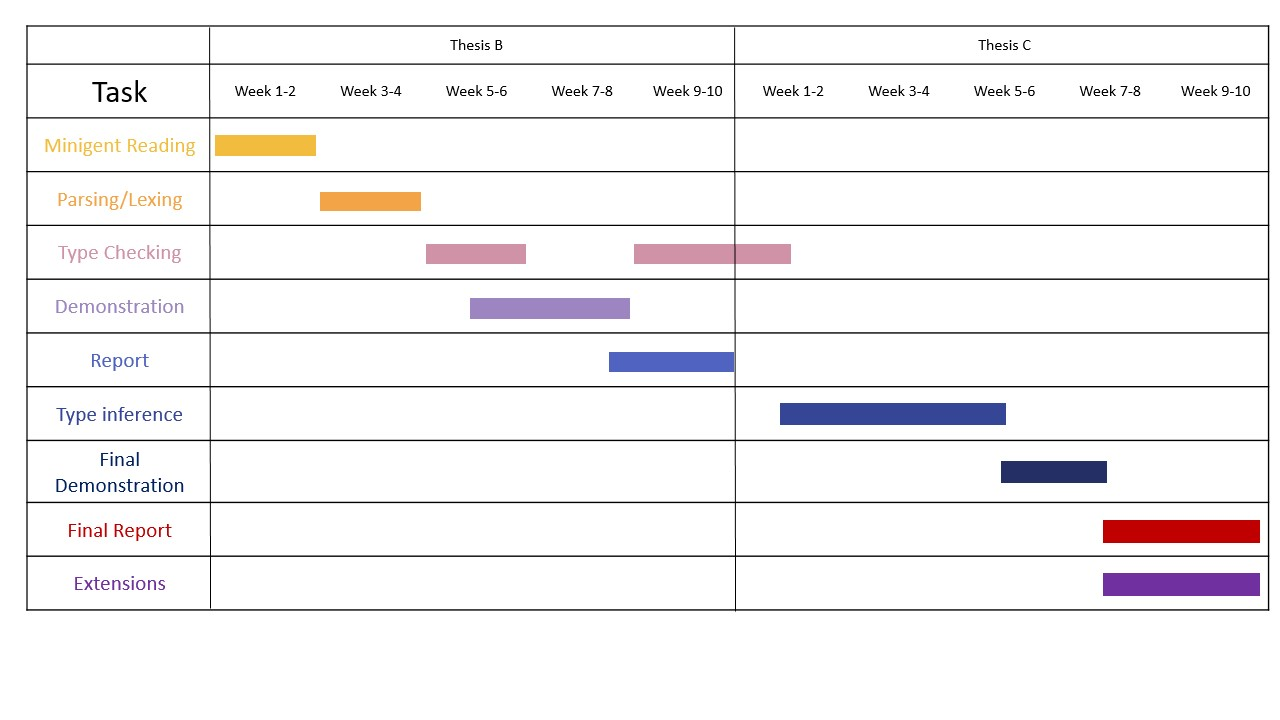
\includegraphics[height=0.55\textheight, angle=90]{content/previous_plan.jpg}
    \caption{The timeline for the project}
    \label{fig:thesisATimeline}
\end{figure}